\documentclass[a4paper, 12pt]{article}
\usepackage{polski}
\usepackage[cp1250]{inputenc}
\usepackage{graphicx}
\usepackage{latexsym}
\author{KG, KK, PP}

\title{Rozprzestrzenianie się fali dźwiękowej po pomieszczeniu}

\author{Kacper Gawroński \and Krzysztof Kogut \and Paweł Perończyk \\
		\small Informatyka, II rok \\
		\small Rok akademicki 2018/19 \\
		}

\begin{document}
\maketitle

\section{Wprowadzenie do tematu}

Rozchodzenie się dźwięku w pomieszczeniu zależy od jego wymiarów i kształtu oraz od struktury powierzchni ograniczającej pomieszczenia, jak też od właściwości akustycznych przedmiotów w niej się znajdujących (co pomijamy z uwagi na potrzeby symulacji). Wymienione czynniki mają wpływ na prędkość zanikania energii dźwiękowej w pomieszczeniu, co z kolei wpływa w sposób zasadniczy na wartość poziomu dźwięku w nim panującego. 
\\ \\
Fale dźwiękowe rozchodzące się w pomieszczeniach natrafiając na przeszkody mogą się od nich odbić. Te odbicia mogą mieć charakter lustrzany (kąt padania jest równy kątowi odbicia) lub też łączyć się z rozproszeniem dźwięku (fala padająca pod określonym kątem jest odbijana we wszystkich kierunkach). To, jaki charakter będzie miało odbicie zależy od relacji między długością fali a rozmiarami elementów rozpraszających. W praktyce, ze względu na duży zakres długości fal dźwiękowych (w zależności od częstotliwości od 1,7 mm do 17 m), zwykle mamy do czynienia z odbiciem mieszanym – składowe dźwięku o pewnych częstotliwościach ulegają odbiciu z rozproszeniem a inne odbiciu lustrzanemu. 
\\ \\
Podczas rozchodzenia się dźwięku w powietrzu następują lokalne zmiany ciśnienia, polegające na odchyleniach powyżej i poniżej normalnego ciśnienia atmosferycznego, czyli ściśnięciach i rozprężenia cząsteczek powietrza. Zwykłe zmiany ciśnienia atmosferycznego, np. związane z pogodą lub wysokością, są zbyt powolne, aby słuch ludzki postrzegał je jako dźwięki. Częstotliwości poniżej około 16-20 cykli na sekundę, czyli herców (1 Hz=1/s), są dla człowieka niesłyszalne, choć czasem ucho na nie reaguje. Te częstotliwości to tzw. infradźwięki. Zakres częstotliwości od około 20 do około 20000 Hz to częstotliwości słyszalne dla człowieka. Dokładny zakres słyszalności jest różny dla różnych osób. Częstotliwości z zakresu słyszalności są postrzegane jako dźwięk, mający określoną wysokość, czy też charakter tonalny albo szumowy. Częstotliwości powyżej 20 kHz nazywamy ultradźwiękami. 
\\ \\
Fala dźwiękowa wychodząca ze źródła dźwięku słabnie wraz ze wzrostem pokonanej odległości od źródła. Osłabienie to zależy od właściwości kierunkowych źródła i od środowiska, w którym ta fala się rozchodzi. Gdy źródło dźwięku jest małe w porównaniu z długością promieniowanej fali, dźwięk rozchodzi się na zewnątrz w formie sfery o promieniu rosnącym wraz z oddalaniem się od źródła. Ponieważ energia dźwięku jest rozprowadzana równomiernie na powierzchni sfery, intensywność dźwięku jest proporcjonalna do odległości od źródła zgodnie z zależnością:

\begin{center}
$\frac{I_{1}}{I_{2}} = \frac{r_{2}^{2}}{r_{1}^{2}}$
\end{center}

gdzie $r_{1}, r_{2}$ - odległości od źródła dźwięku, $I_{1}, I_{2}$ - intensywność dźwięku w odległości odpowiednio: $r_{1}$ i $r_{2}$. Odpowiada to zmniejszeniu poziomu o 6 dB przy podwojeniu odległości. 
\\ \\
Wynika to z niezakłóconego, przestrzennego rozproszenia energii dźwiękowej. We wnętrzach jest nieco inaczej. Poziom dźwięku opada w podobnym tempie w najbliższym otoczeniu źródła, tam gdzie dominuje dźwięk bezpośredni tego źródła (czyli w tzw. polu bezpośrednim). Pozostała przestrzeń w pomieszczeniu jest tzw. polem pogłosowym, gdzie dominują dźwięki odbite. Poziom dźwięku w polu pogłosowym wszędzie jest taki sam lub bardzo zbliżony. Stąd zanik przestrzenny dźwięku w pomieszczeniach jest zwykle dużo słabszy niż w przestrzeni otwartej.
\\ \\

\section{Przegląd literatury}

Istnieje wiele możliwości badania rozchodzenia się fal dźwiękowych. Począwszy od rzeczywistych przyrządów stworzonych w celach naukowych do generowania dźwięku, przez przedmioty codziennego użytku, aż po aplikacje internetowe lub na telefon.
\\ \\ 
Jednym ze sposobów mierzenia rozchodzenia się dźwięku jest wykorzystanie obrabiarki \footnote{\textit{Badania własności obrabiarek i stosowane kryteria oceny} dr inż Wacław Skoczyński, Przegląd Mechaniczny, 2003} generującej dźwięk o dużym natężeniu. Umieszczona w pomieszczeniu, w którym znajduje się swobodne pole akustyczne, a własności akustyczne podłoża są jednakowe (lub bardzo zbliżone) na powierzchni ograniczonej położeniem punktów pomiarowych i pozwalających traktowanie ich jako odbijających hałas. Punkty pomiarowe są rozmieszczone na powierzchniach prostopadłościanu, którego ściany otaczają obrabiarkę (lub tę jej część, którą można uznać za główne źródło dźwięku) w odległości 1 - 1,5 m. W każdym punkcie pomiarowym ustawiamy mikrofon bezpośrednio w stronę źródła dźwięku i wykonujemy pomiar.
\\ \\
W dzisiejszych czasach mamy jednak do czynienia w większości z aplikacjami internetowymi lub na telefony komórkowe, które służą do pomiaru dźwięku. \footnote{\textit{Miernik dźwięku (Sound Meter)} Abc Apps} Aplikacja \textit{Sound Meter} wykorzystuje mikrofony w urządzeniach z systemem Android do wychwytywania dźwięku z otoczenia i mierzenia jego natężenia. Miernik ten może być wykorzystany podczas badania postawionego wyżej problemu rozchodzenia się fali dźwiękowej. Wystarczy obrać konkretną odległość źródła dźwięku od telefonu z aplikacją. Trzeba jednak dopilnować, aby na drodze fali dźwiękowej, którą zamierzamy wysłać nie pojawiła się żadna przeszkoda - doprowadzi ona do zniekształcenia fali i błędnych wyników. Trzeba wziąć pod uwagę fakt, że mikrofony dostępne w urządzeniach komórkowych są ograniczone i dostosowane do natężenia dźwięku o wartości 0 - 100 dB. Każda wartość wychodząca poza ten przedział nie będzie rozpoznana i nie otrzymamy pożądanego wyniku.
\\ \\
Istnieje również wiele symulatorów akustycznych pomieszczeń \footnote{\textit{Soundtracing w grach komputerowych} Bugiel P. Kraków, 2013}, wykorzystujących środowisko programu MATLAB. Pozwala to na bardzo dokładne zasymulowanie zjawiska wraz z czynnikami takimi jak pochłanianie dźwięku przez atmosferę \footnote{\textit{Wibroakustyka stosowana.} Cempel C. Warszawa, PWN 1989}, pokrycie materiałem podłogi pomieszczenia, czy spadek ciśnienia wraz z odległością od źródła \footnote{\textit{Dźwięki i fale.} Makarewicz R. Poznań, Wydawnictwo Naukowe UAM 2004}. Gotowy symulator generuje odpowiedzi impulsowe pomieszczenia biorąc pod uwagę najważniejsze zjawiska zachodzące w czasie propagacji dźwięku. Ograniczeniem w tych symulacjach jest częstotliwość próbkowania, która musi być taka sama lub bardzo zbliżona do tej zadanej jako argument symulatora.
\\ \\
W środowisku naukowym popularna okazuje się być metoda FDTD \footnote{\textit{Application of finite difference time domain (FDTD) simulations in engineering education in optics and electrodynamic} Krawszewski M. Politechnika Gdańska, 2013}(Finite Difference Time Domain) - czyli metoda rozwiązywania równań Maxwella w dziedzinie czasu za pomocą różnic skończonych. Symulacje metodą FDTD znalazły zastosowanie w omawianiu takich zagadnień jak rozpraszanie światła, interferencja oraz dyfrakcja fal \footnote{\textit{Efficient and Accurate Sound Propagation
Using Adaptive Rectangular Decomposition} Nikunj Raghuvanshi, Rahul Narain, Ming C. Lin, 2009} dźwiękowych. Jest to prosta w implementacji metoda dająca możliwość wizualizacji przebiegu zjawisk fizycznych zarówno tych wymienionych wcześniej jak i wielu innych.
\\ \\
Innym modelem rozwiązania tego problemu jest metoda wymagająca zastosowania numerycznej symulacji wykorzystującej FSI(Fluid Structure Interaction) \footnote{\textit{Acoustic Intensity Imaging Methods for in-situ Wave Propagation} Stefan Weyna Zachodniopomorski Uniwersytet Technologiczny, Szczecin 2010}. Modelowanie tą metodą wymaga zarówno reprezentacji strukturalnej cieczy, tudzież powietrza oraz związków pomiędzy cząsteczkami. Jest to bardzo trudna metoda w zastosowaniu, wymagająca dużej precyzji w opisach matematycznych, jednakże jest to metoda dająca bardzo dokładne i zbliżone do rzeczywistości wyniki. 
\\

\section{Proponowany model}

W swojej symulacji wykorzystaliśmy zasadę działania automatów komórkowych \footnote{\textit{Visualization of sound propagation and scattering in rooms} Takatoshi Yokota, Shinichi Sakamoto, Hideki Tachibana}. Symulacja propagacji fali dźwiękowej przeprowadzona została poprzez stany komórek oraz ich interakcję z sąsiednimi komórkami. Każda komórka stanowi osobny obiekt, a atrybuty kolejno oddalonych od źródła komórek są obliczane na podstawie sąsiednich komórek - po to aby pomiary były obarczone jak najmniejszym błędem związanym z ich predykcją u źródła dźwięku. 
\\

\section{Symulacja zjawiska}

Nasza symulacja została wykonana w języku programowania - Pythonie z wykorzystaniem bibliotek: Matplotlib i Numpy. 
\\ \\
Idea operacji wykonywanych na komórkach jest bardzo prosta, każda komórka zawiera informacja o obecnej wartości ciśnienia oraz natężeniu przepływu powietrza. W każdym kolejnym kroku symulacji obliczamy nowe wartości ciśnienia oraz natężenia przepływu powietrza bazując na poprzednich wartościach.
\\ \\
Symulację przeprowadzamy w środowisku 2D. Pierwszym krokiem jest obliczenie początkowego pływu powietrza dla wszystkich komórek - przy jednoczesnej znajomości różnicy ciśnień. Obliczamy prędkość przepływu powietrza w każdej komórce na podstawie różnicy wartości ciśnień panującymi pomiędzy komórką i jej sąsiadami.
\\ \\
Używając określenia wpływ/wypływ powietrza mówimy tutaj o parametrach powietrza w momencie wkraczania/wychodzenia z konkretnej komórki, czyli przepływ powietrza, tzw. flow to przedstawienie powietrza jako określonych co do wartości atrybutów, w tym wypadku - ciśnienie i prędkość.

\begin{verbatim}
for i in range(size_y):
  for j in range(size_x):
    if wall[i][j] == 1:
      V[i][j][0] = V[i][j][1] = V[i][j][2] = V[i][j][3] = 0.0
      continue
    cellPressure = P[i][j]
		
    if i > 0 
      V[i][j][0] = V[i][j][0] + cellPressure - P[i - 1][j] 
    else cellPressure
		
    if j < size_x - 1 
      V[i][j][1] = V[i][j][1] + cellPressure - P[i][j + 1] 
    else cellPressure

    if i < size_y - 1 
      V[i][j][2] = V[i][j][2] + cellPressure - P[i + 1][j]
    else cellPressure
		
    if j > 0 
      V[i][j][3] = V[i][j][3] + cellPressure - P[i][j - 1]  
    else cellPressure
\end{verbatim}

Następnie symulujemy już przepływ, czyli aktualizujemy ciśnienie biorąc pod uwagę również prędkość wypływu powietrza(outflow velocity):

\begin{verbatim}
for i in range(size_y):
  for j in range(size_x):

    self.pressure[i][j] -= 0.5 * damping * sum(self.velocities[i][j])
\end{verbatim}

Żeby przeprowadzić symulację należy ustawić poniższe parametry: 
\begin{itemize}
\item scale(skala)
\item damping(tłumienie)
\item omega(parametr używany przy obliczaniu falowego sygnału źródła)
\item startPressure(ciśnienie początkowe)
\item yPosition(współrzędna Y źródła)
\item xPosition(współrzędna X źródła)\\
\end{itemize}

Następnie w wywołać przy pomocy poniższego kodu w linii komend: \\

\begin{verbatim}
python main.py [wall_option] [single | multi]
\end{verbatim}

\hspace{1.5cm} gdzie: \textbf{wall\_option} -- oznacza liczbę 1--9 (single) lub 1--8 (multi)

\begin{center}
\emph{lub}
\end{center}

\begin{verbatim}
python main.py [-h | --help]
\end{verbatim}

\hspace{1.5cm} w celu uzyskania pomocy \\



\section{Wyniki symulacji}

Poniżej przedstawione zostały różne wyniki symulacji.

\newpage


\begin{figure}
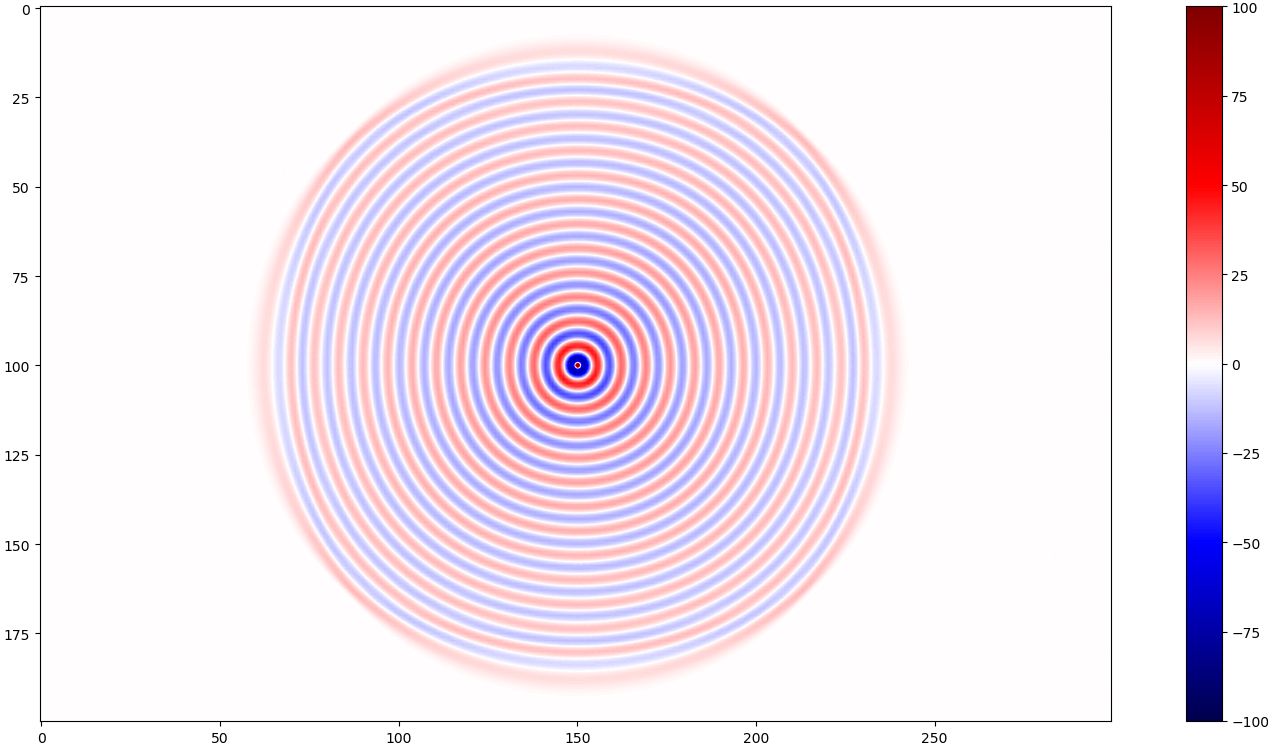
\includegraphics[scale=0.43]{no1.png}
\caption{Swobodne rozchodzenie się fali z jednym źródłem}
\end{figure}

\begin{figure}
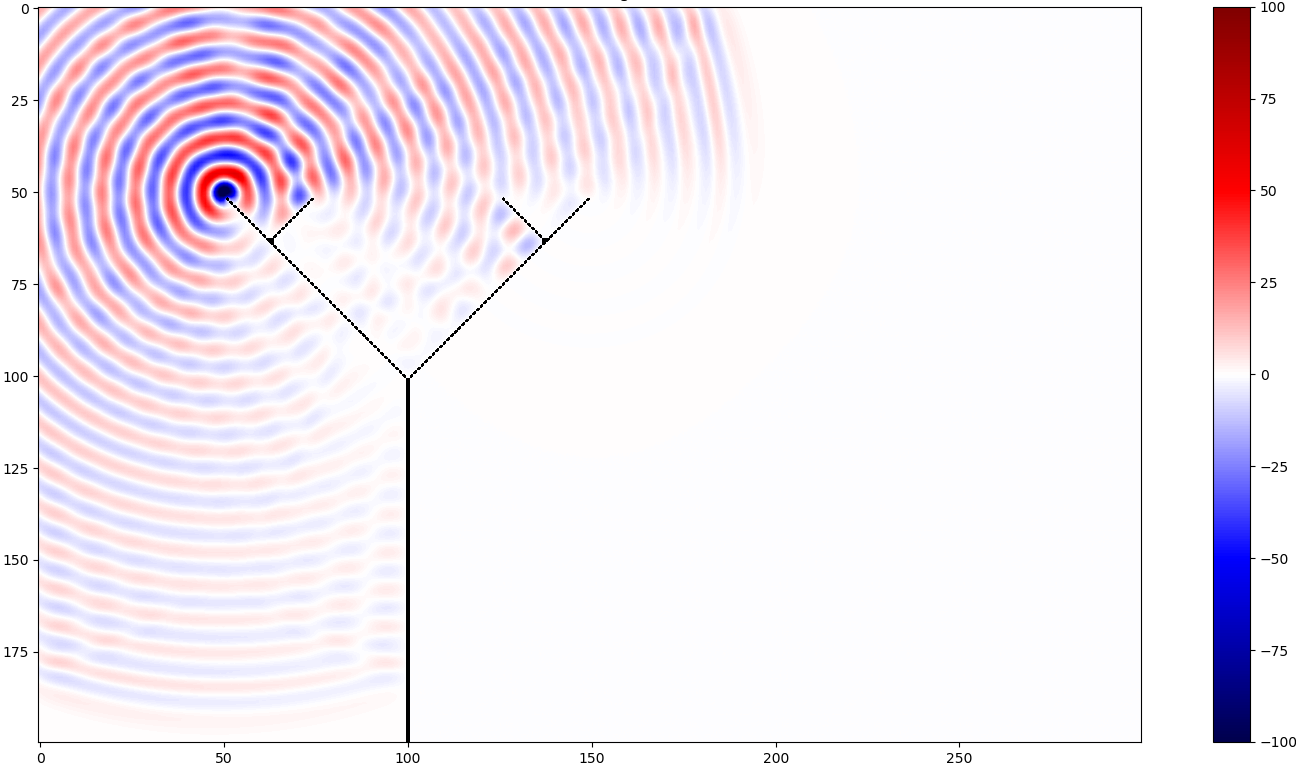
\includegraphics[scale=0.43]{no2.png}
\caption{Fala dźwiękowa ze źródłem na zewnątrz przeszkody}
\end{figure}

\begin{figure}
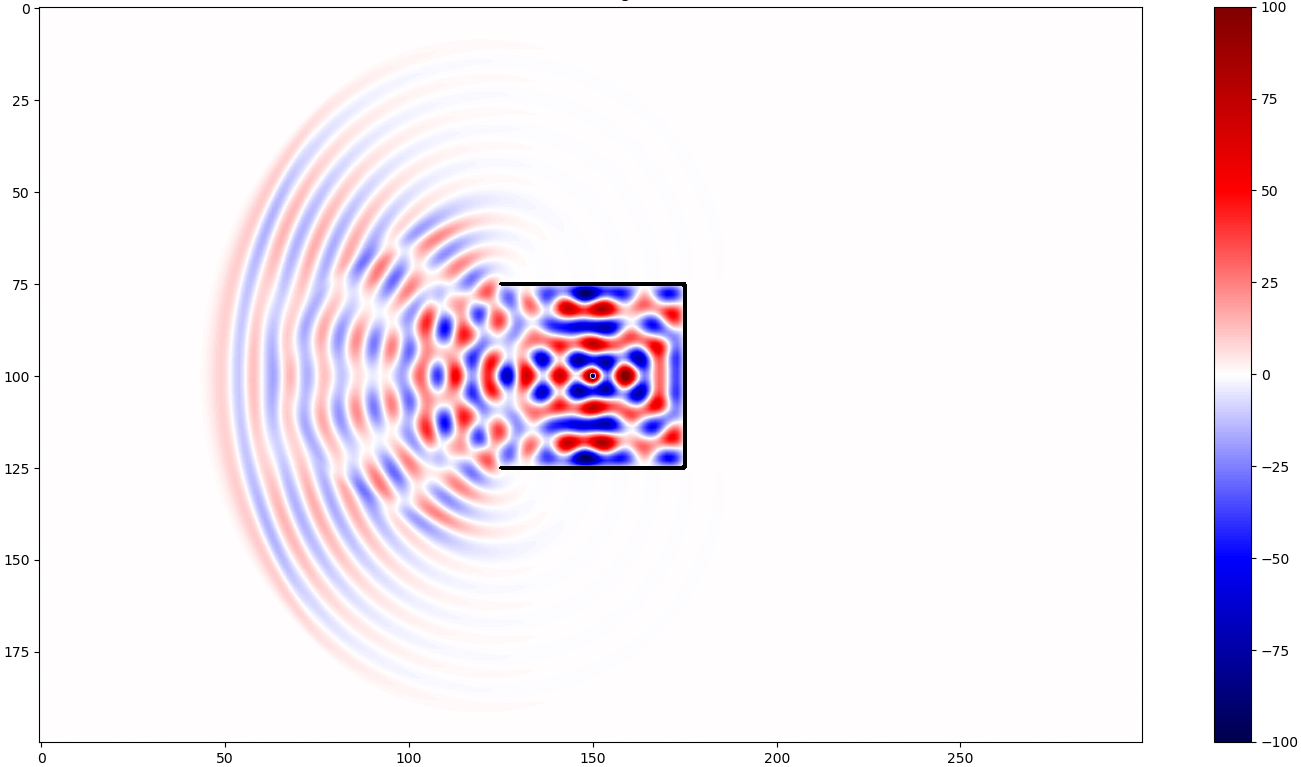
\includegraphics[scale=0.43]{no3.png}
\caption{Fala dźwiękowa ze źródłem wewnątrz przeszkody}
\end{figure}

\begin{figure}
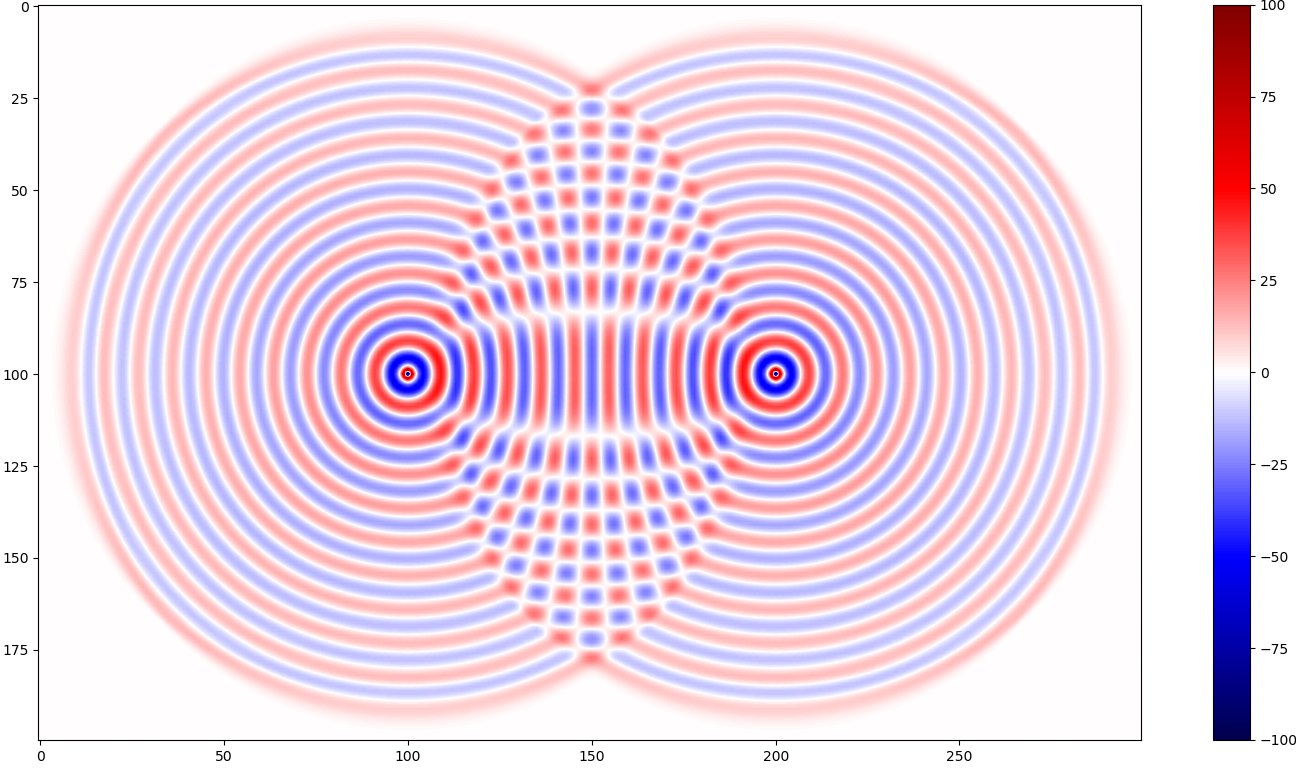
\includegraphics[scale=0.43]{no4.png}
\caption{Dwa źródła fal dźwiękowych nachodzących na siebie}
\end{figure}

\begin{figure}
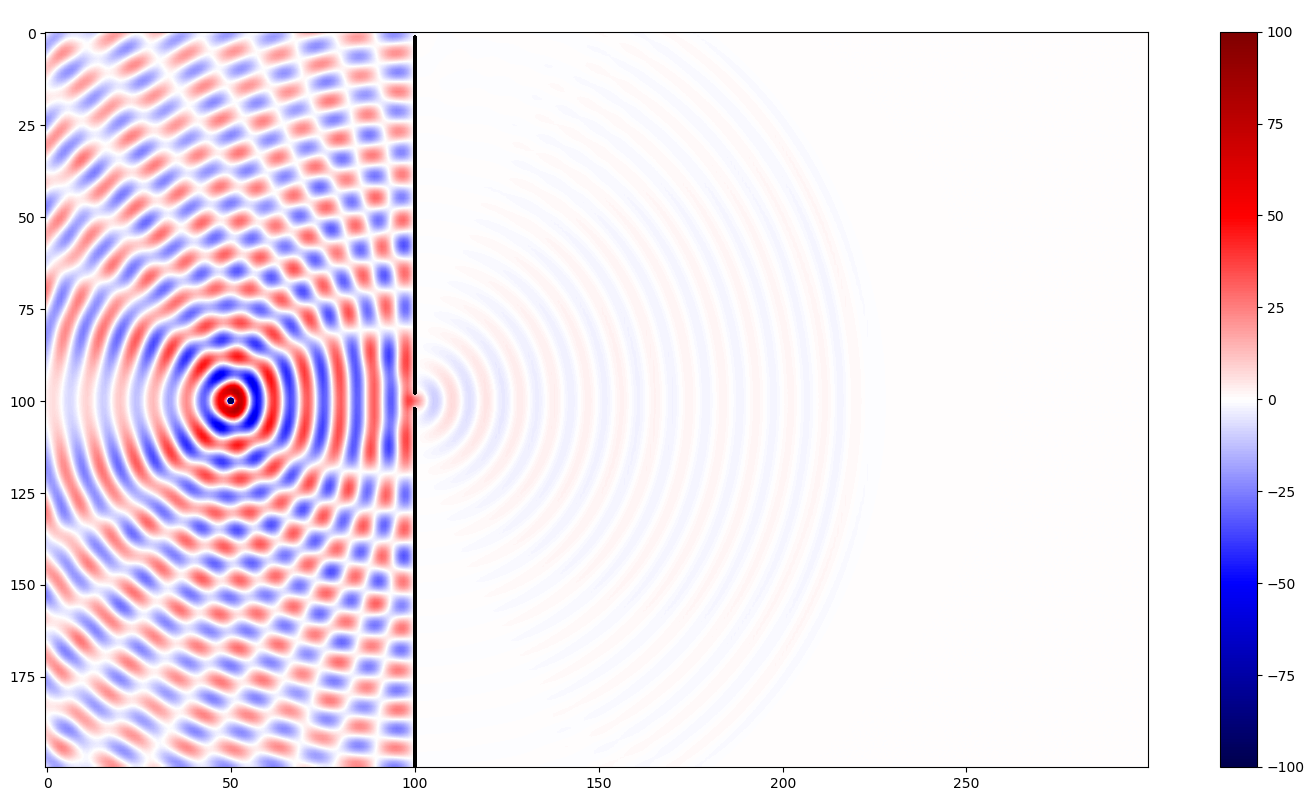
\includegraphics[scale=0.55]{no5.png}
\caption{Zjawisko dyfrakcji(ugięcia) fali dźwiękowej zachodzące przy przejściu przez szczelinę}
\end{figure}



\begin{figure}
\section{Wnioski}

Problem symulacji fali dźwiękowej ma szereg rozwiązań bardziej lub mniej dokładnych. Pierwszym krokiem do rozwiązania tego problemu jest określenie do jakich celów ma służyć symulacja. Jeżeli problem ma podłoże naukowe powinno się zastosować bardziej dokładne i czasochłonne metody, które nie tyle ukazują nam sam obraz, ale szereg działań i zależności zachodzących podczas propagacji fali dźwiękowej. Natomiast zobrazowanie fali dźwiękowej na potrzeby zobrazowania samego w sobie nie wymaga bardzo dokładnych metod obliczeniowych. Biorąc pod uwagę symulacje, które zostały przeprowadzone i te zaprezentowane na powyższych ilustracjach można śmiało stwierdzić, że rozwiązanie problemu zaproponowanym przez nas algorytmem jest wystarczająco dokładne i wiarygodne, co potwierdza fakt występowania zjawisk dyfrakcji i interferencji fali dźwiękowej - co oddaje rzeczywisty obraz dźwięku w przestrzeni.

\end{figure}


\end{document}
